%%%%%%%%%%%%%%%%%%%%%%%%%%%%%%%%%%%%%%%%%
% Short Sectioned Assignment LaTeX Template Version 1.0 (5/5/12)
% This template has been downloaded from: http://www.LaTeXTemplates.com
% Original author:  Frits Wenneker (http://www.howtotex.com)
% License: CC BY-NC-SA 3.0 (http://creativecommons.org/licenses/by-nc-sa/3.0/)
%%%%%%%%%%%%%%%%%%%%%%%%%%%%%%%%%%%%%%%%%

%----------------------------------------------------------------------------------------
%	PACKAGES AND OTHER DOCUMENT CONFIGURATIONS
%----------------------------------------------------------------------------------------

\documentclass[paper=a4, fontsize=11pt]{scrartcl} % A4 paper and 11pt font size

% ---- Entrada y salida de texto -----

\usepackage[T1]{fontenc} % Use 8-bit encoding that has 256 glyphs
\usepackage[utf8]{inputenc}
%\usepackage{fourier} % Use the Adobe Utopia font for the document - comment this line to return to the LaTeX default

% ---- Idioma --------

\usepackage[spanish, es-tabla]{babel} % Selecciona el español para palabras introducidas automáticamente, p.ej. "septiembre" en la fecha y especifica que se use la palabra Tabla en vez de Cuadro

% ---- Otros paquetes ----

\usepackage{url} % ,href} %para incluir URLs e hipervínculos dentro del texto (aunque hay que instalar href)
\usepackage{amsmath,amsfonts,amsthm} % Math packages
%\usepackage{graphics,graphicx, floatrow} %para incluir imágenes y notas en las imágenes
\usepackage{graphics,graphicx, float} %para incluir imágenes y colocarlas

% Para hacer tablas comlejas
%\usepackage{multirow}
%\usepackage{threeparttable}

%\usepackage{sectsty} % Allows customizing section commands
%\allsectionsfont{\centering \normalfont\scshape} % Make all sections centered, the default font and small caps

\usepackage{fancyhdr} % Custom headers and footers

\pagestyle{fancyplain} % Makes all pages in the document conform to the custom headers and footers
\fancyhead{} % No page header - if you want one, create it in the same way as the footers below
\fancyfoot[L]{} % Empty left footer
\fancyfoot[C]{} % Empty center footer
\fancyfoot[R]{\thepage} % Page numbering for right footer
\renewcommand{\headrulewidth}{0pt} % Remove header underlines
\renewcommand{\footrulewidth}{0pt} % Remove footer underlines
\setlength{\headheight}{13.6pt} % Customize the height of the header

\numberwithin{equation}{section} % Number equations within sections (i.e. 1.1, 1.2, 2.1, 2.2 instead of 1, 2, 3, 4)
\numberwithin{figure}{section} % Number figures within sections (i.e. 1.1, 1.2, 2.1, 2.2 instead of 1, 2, 3, 4)
\numberwithin{table}{section} % Number tables within sections (i.e. 1.1, 1.2, 2.1, 2.2 instead of 1, 2, 3, 4)

\setlength\parindent{0pt} % Removes all indentation from paragraphs - comment this line for an assignment with lots of text

\newcommand{\horrule}[1]{\rule{\linewidth}{#1}} % Create horizontal rule command with 1 argument of height
\usepackage[breaklinks=true]{hyperref}

\usepackage[dvipsnames]{xcolor}
\usepackage{amssymb}
\usepackage{color}
\usepackage{listings}
\usepackage{upgreek} % para poner letras griegas sin cursiva
\usepackage{cancel} % para tachar
\usepackage{mathdots} % para el comando \iddots
\usepackage{mathrsfs} % para formato de letra
\usepackage{stackrel} % para el comando \stackbin
\lstset{ %
language=C++,                % elegir el lenguaje del código
stringstyle=\color{blue}\ttfamily,,
basicstyle=\normalsize\ttfamily,       % el tamaño del font a usar para el código
numbers=left,                   % dónde poner los números de línea 
numberstyle=\footnotesize,      % tamaño de font usados para los números de línea 
stepnumber=1,                   % el paso de numeración
numbersep=5pt,                  % distancia del numero de línea y la línea
backgroundcolor=\color{white},  % color de fondo, para usarlo hay que agregar  \usepackage{color}
showspaces=false,               % mostrar espacios en blanco ?
showstringspaces=false,         % subrayar espacios con cadenas?   
 showtabs=false,                 % mostrar taba usando cadenas? 
frame=single,           			% enmarcar el código?  
tabsize=2,          				% sets default tabsize to 2 spaces?
keywordstyle=\color{MidnightBlue}\ttfamily\bfseries,
commentstyle=\color{OliveGreen}\ttfamily,
morecomment=[l][\color{OliveGreen}]{\#},
captionpos=b,           % sets the caption-position to bottom?
breaklines=true,        % sets automatic line breaking?
breakatwhitespace=false,    % sets if automatic breaks should only happen at whitespace ?
title=\lstname,
escapeinside={\%*}{*)}          % if you want to add a comment within your code
}

\lstset{literate=
  {á}{{\'a}}1 {é}{{\'e}}1 {í}{{\'i}}1 {ó}{{\'o}}1 {ú}{{\'u}}1
  {Á}{{\'A}}1 {É}{{\'E}}1 {Í}{{\'I}}1 {Ó}{{\'O}}1 {Ú}{{\'U}}1
  {à}{{\`a}}1 {è}{{\`e}}1 {ì}{{\`i}}1 {ò}{{\`o}}1 {ù}{{\`u}}1
  {À}{{\`A}}1 {È}{{\'E}}1 {Ì}{{\`I}}1 {Ò}{{\`O}}1 {Ù}{{\`U}}1
  {ä}{{\"a}}1 {ë}{{\"e}}1 {ï}{{\"i}}1 {ö}{{\"o}}1 {ü}{{\"u}}1
  {Ä}{{\"A}}1 {Ë}{{\"E}}1 {Ï}{{\"I}}1 {Ö}{{\"O}}1 {Ü}{{\"U}}1
  {â}{{\^a}}1 {ê}{{\^e}}1 {î}{{\^i}}1 {ô}{{\^o}}1 {û}{{\^u}}1
  {Â}{{\^A}}1 {Ê}{{\^E}}1 {Î}{{\^I}}1 {Ô}{{\^O}}1 {Û}{{\^U}}1
  {œ}{{\oe}}1 {Œ}{{\OE}}1 {æ}{{\ae}}1 {Æ}{{\AE}}1 {ß}{{\ss}}1
  {ű}{{\H{u}}}1 {Ű}{{\H{U}}}1 {ő}{{\H{o}}}1 {Ő}{{\H{O}}}1
  {ç}{{\c c}}1 {Ç}{{\c C}}1 {ø}{{\o}}1 {å}{{\r a}}1 {Å}{{\r A}}1
  {€}{{\EUR}}1 {£}{{\pounds}}1
  {ñ}{{\~n}}1
}



\hypersetup{
    colorlinks=true,
    linkcolor=black,
    filecolor=magenta,      
    urlcolor=blue,
    pdftitle={ED: Práctica 3 - Mario Rodríguez Ruiz},
    bookmarks=true,
}



%----------------------------------------------------------------------------------------
%	TÍTULO Y DATOS DEL ALUMNO
%----------------------------------------------------------------------------------------

\title{	
\normalfont \normalsize 
\textsc{\textbf{Estructura de Datos (2016-2017)} \\ Subgrupo C2 \\ Grado en Ingeniería Informática\\ Universidad de Granada} \\ [25pt] % Your university, school and/or department name(s)
\horrule{0.5pt} \\[0.4cm] % Thin top horizontal rule
\huge Práctica 1: Eficiencia \\ % The assignment title
\horrule{2pt} \\[0.5cm] % Thick bottom horizontal rule
}

\author{Mario Rodríguez Ruiz} % Nombre y apellidos

\date{\normalsize\today} % Incluye la fecha actual

%----------------------------------------------------------------------------------------
% DOCUMENTO
%----------------------------------------------------------------------------------------

\begin{document}

\maketitle % Muestra el Título

\newpage %inserta un salto de página

\tableofcontents % para generar el índice de contenidos

\listoffigures

\listoftables

\newpage

%----------------------------------------------------------------------------------------
%	Cuestión 0
%----------------------------------------------------------------------------------------

\section{Información del ordenador}

Portatil ASUS X75A


%------------------------------------------------

\subsection{Hardware}
\begin{figure}[H] %con el [H] le obligamos a situar aquí la figura
\centering
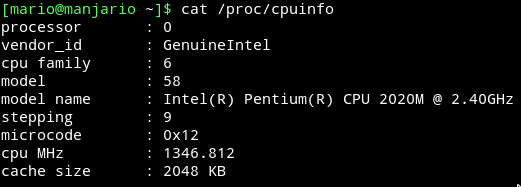
\includegraphics[scale=0.756]{ejercicio0/cpu.png}  %el parámetro scale permite agrandar o achicar la imagen. En el nombre de archivo puede especificar directorios
\caption{Información del CPU.} 
\label{fig:figura1.1}
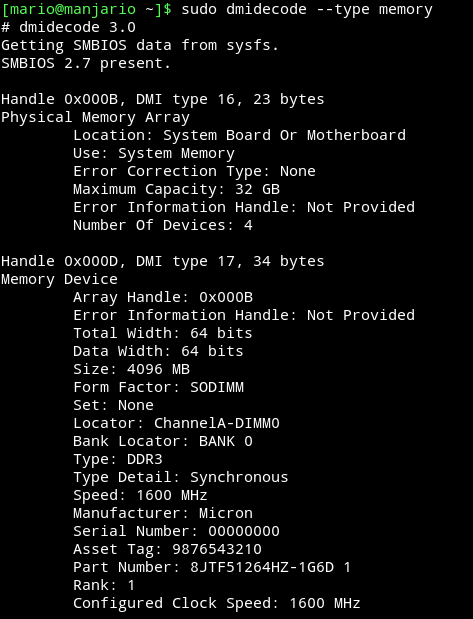
\includegraphics[scale=0.7]{ejercicio0/mem1.png}  %el parámetro scale permite agrandar o achicar la imagen. En el nombre de archivo puede especificar directorios
\caption{Módulo 1 de memoria RAM.} 
\label{fig:figura1.2}
\end{figure}

\begin{figure}[H] %con el [H] le obligamos a situar aquí la figura
\centering
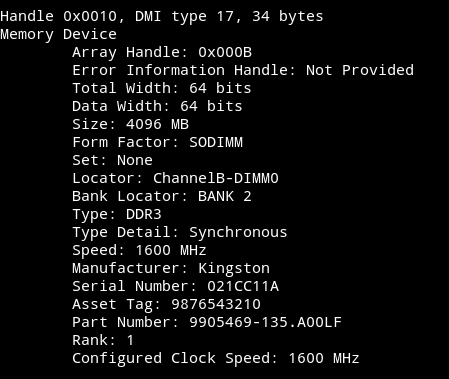
\includegraphics[scale=0.7]{ejercicio0/mem2.png}  %el parámetro scale permite agrandar o achicar la imagen. En el nombre de archivo puede especificar directorios
\caption{Módulo 2 de memoria RAM.} 
\label{fig:figura1.3}
\end{figure}

\subsection{Sistema operativo}
\begin{figure}[H] %con el [H] le obligamos a situar aquí la figura
\centering
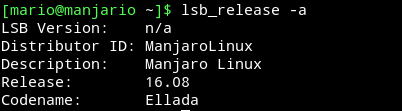
\includegraphics[scale=1]{ejercicio0/SO.png}  %el parámetro scale permite agrandar o achicar la imagen. En el nombre de archivo puede especificar directorios
\caption{Información del SO.} 
\label{fig:figura1}
\end{figure}

\subsection{Compilador}
\begin{figure}[H] %con el [H] le obligamos a situar aquí la figura
\centering
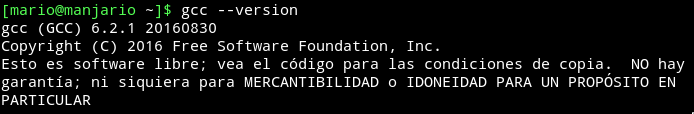
\includegraphics[scale=0.6]{ejercicio0/compilador.png}  %el parámetro scale permite agrandar o achicar la imagen. En el nombre de archivo puede especificar directorios
\caption{Información del compilador.} 
\label{fig:figura2}
\end{figure}

\newpage

%----------------------------------------------------------------------------------------
%	Cuestión 1
%----------------------------------------------------------------------------------------

\section{Ejercicio 1: Ordenación de la burbuja}

\subsection{Cálculo de la eficiencia teórica y empírica de/con el algoritmo de la burbuja}

\begin {lstlisting}
void ordenar(int *v, int n) {						
	for (int i=0; i<n-1; i++)						
		for (int j=0; j<n-i-1; j++)
			if (v[j]>v[j+1]) {									
				int aux = v[j];		
				v[j] = v[j+1];						
				v[j+1] = aux;
			}
}
\end{lstlisting}

\begin{itemize}
	\item Linea 2: 3 OE (asignación, decremento, comparación) + 1 OE
	\item Linea 3: 4 OE (asignación, 2 decrementos, comparación) + 1 OE	
	\item Linea 4: 4 OE (2 accesos al elemento v[j], incremento, comparación)
	\item Linea 5: 2 OE (acceso al elemento v[j], asignación)
	\item Linea 6: 4 OE (2 accesos al elemento v[j], incremento, asignación)
	\item Linea 7: 3 OE (acceso al elemento v[j], incremento, asignación)
\end{itemize}

Bucle de la j
\begin{equation}
Tj (n)= \sum_{j=0}^{n-i-1}17 = 17 n-17i
\end{equation}

Bucle de la i
\begin{equation}
Ti (n)= \sum_{i=0}^{n-1}(1+17n-17i) = \sum_{i=0}^{n-1}1 + \sum_{i=0}^{n-1}17n - \sum_{i=0}^{n-1}17i = n+17n^2+17 \frac{n(n+1)}{2}	
\end{equation}
\begin{equation}
 Ti(n) = \frac12 (51n^2 + 19n)
\end{equation}
\begin{equation}
\textup{Por lo que el orden de eficiencia de la función es de }  O(n^2)
\end{equation}

\newpage
---
\subsection{Experimento con el algoritmo de la burbuja}
\lstinputlisting{ejercicio1/ordenacion.cpp}
\lstinputlisting{ejercicio1/ejecuciones_ordenacion.csh}
\newpage

Los resultados, una vez analizados y procesados por gnuplot son los mostrados en
la Figura~\ref{fig:figura1-1}. Como se puede comprobar, el gráfico muestra un resultado en forma parabólica, coincidiendo con el estudio teórico.

\begin{figure}[H] %con el [H] le obligamos a situar aquí la figura
\centering
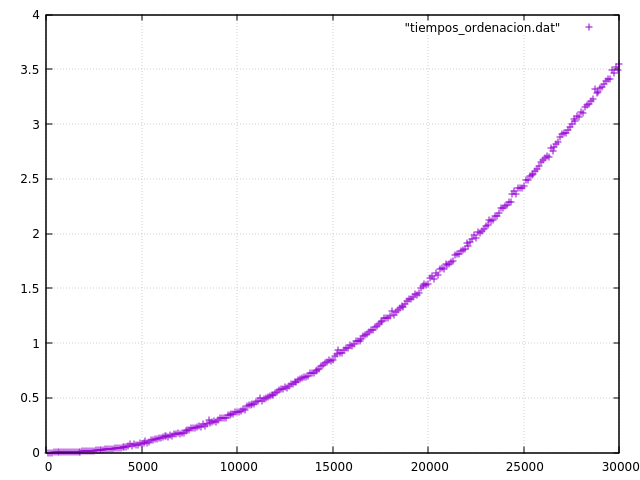
\includegraphics[scale=0.6]{ejercicio1/ejercicio1.png}  %el parámetro scale permite agrandar o achicar la imagen. En el nombre de archivo puede especificar directorios
\caption{Datos dibujados con Gnuplot} 
\label{fig:figura1-1}
\end{figure}
Lo que sucede al superponer ambas eficiencias es que los resultados de ambos coinciden completamente tal y como se puede comprobar en la Figura~\ref{fig:figura1-2}.
\begin{figure}[H] %con el [H] le obligamos a situar aquí la figura
\centering
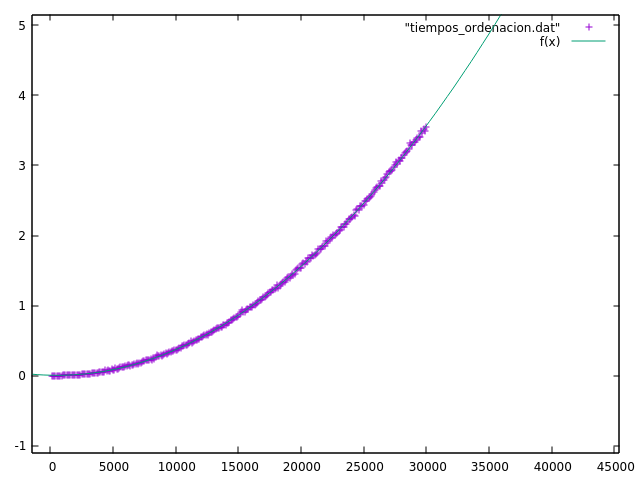
\includegraphics[scale=0.6]{ejercicio1/ejercicio1-2.png}  %el parámetro scale permite agrandar o achicar la imagen. En el nombre de archivo puede especificar directorios
\caption{Superposición eficiencia teórica y empírica} 
\label{fig:figura1-2}
\end{figure}


%----------------------------------------------------------------------------------------
%	Cuestión 2
%----------------------------------------------------------------------------------------
\section{Ejercicio 2: Ajuste en la ordenación de la burbuja}

\begin{figure}[H] %con el [H] le obligamos a situar aquí la figura
\centering
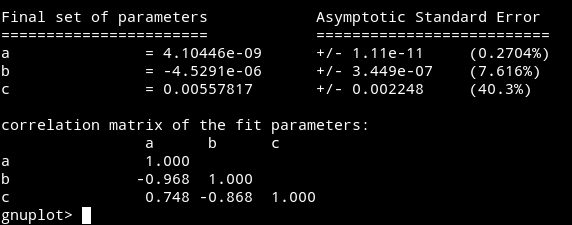
\includegraphics[scale=0.8]{ejercicio2/ejercicio2.png}  %el parámetro scale permite agrandar o achicar la imagen. En el nombre de archivo puede especificar directorios
\caption{Cálculo de a, b y c por gnuplot} 
\label{fig:figura2-0}
\end{figure}

Replicando el experimento anterior, esta vez antes hemos obtenido los valores de a, b y c por medio de gnuplot para que, a continuación, como se ve en la Figura~\ref{fig:figura2-1} superponer ambas eficiencias.
\begin{figure}[H] %con el [H] le obligamos a situar aquí la figura
\centering
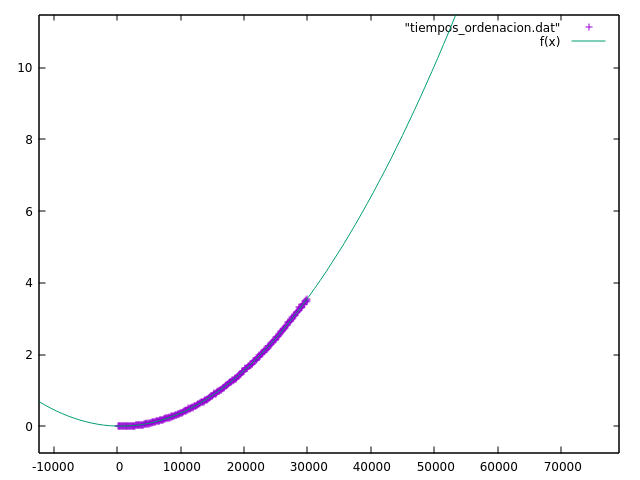
\includegraphics[scale=0.8]{ejercicio2/ejercicio2-1.png}  %el parámetro scale permite agrandar o achicar la imagen. En el nombre de archivo puede especificar directorios
\caption{Superposición eficiencia teórica y empírica} 
\label{fig:figura2-1}
\end{figure}

\newpage
%----------------------------------------------------------------------------------------
%	Cuestión 3
%----------------------------------------------------------------------------------------
\section{Ejercicio 3: Problemas de precisión}
\subsection{Qué hace el algoritmo}
El algoritmo es un común de búsqueda binaria. Este, para su correcto funcionamiento, requiere un vector ordenado en el que busca un valor concreto. 

La característica fundamental de éste es que en cada iteracción va descartando la mitad del vector en la que no se encuentra el valor especificado. Su funcionamiento es el siguiente: compara el valor especificado con el valor del centro del vector; si es mayor el del centro, el valor está en la parte izquierda, en caso contrario estará en la derecha. De esta forma en cada iteración se elimina la mitad del
vector restante. 

\subsection{Eficiencia teórica}
Para este estudio solo es necesario hacer énfasis en la condición del bucle ya que
el resto de instrucciones son de orden constante, por lo que se pueden obviar. 

En cuanto a la condición, se tiene que 
\begin {verbatim}
while ((inf<sup) && (!enc))
\end{verbatim}
siendo el peor de los casos \textbf{(inf<sup)}, lo que produce que \texttt{inf==sup}, es decur, sólamente es necesario quedarse con un elemento. 

Teniendo un vector de \texttt{n elementos}, en la primera iteración se obtendría n, pero en las siguientes iteraciones se tendría \texttt{n/2, n/4, n/8, n/16}... así sucesivamente hasta llegar
a la iteración \texttt{i-esima}. En esta última se obtendrá que \textbf{n/2i <= 1} elementos. 

Por tanto, el número de iteraciones obtenida a raiz de la fórmula obtenida es:

\begin{center}\textbf{n <= 2i}, que en forma logarítmica será:
\textbf{log2 n <= i}\end{center}

Es decir, el bucle se recorrerá en el peor de los casos i veces, siendo i el logaritmo en base 2 de n. 

Finalmente, se concluye que el algoritmo tiene un orden de complejidad \textbf{O(log n)}.

\subsection{Eficiencia empírica}
Un problema que puede ocasionar un algoritmo tan eficiente como éste es la dificultad para medir tiempos tan bajos. Una solución podría ser la utilización de vectores muy grandes, pero aún así el algoritmo lo solucionaría de forma idéntica. Lo que además ocurre es que para tamaños pequeños el tiempo aumenta muy rápido y, para tamaños grandes muy despacio. Por ello es que se tengan que hacer esos incrementos siempre en función del tamaño.

Para realizar una medición que solucione los problemas anteriores se proponen dos cambios:
\begin{enumerate}
	\item Uso de la clase \textbf{high\_resolution\_clock} de la biblioteca \textbf{<chrono>}
	
	Ésta permite hacer mediciones en \textbf{nanosegundos}.
	\lstinputlisting{ejercicio3/ejercicio_desc.cpp}
	\item Ejecución mediante un script que incrementa los tamaños lentamente al principio y brúscamente, al superar el crecimiento exponencial de la curva. 
	\lstinputlisting{ejercicio3/ejecuciones_desc.csh}
	
\subsection{Ajuste de la eficiencia teórica}
	
	Para calcular a y b (Figura~\ref{fig:figura3-1}) en este apartado se ejecuta lo siguiente en \textbf{gnuplot}:
	
\textbf{f(x) = a*log(x) + b}

\begin{figure}[H] %con el [H] le obligamos a situar aquí la figura
\centering
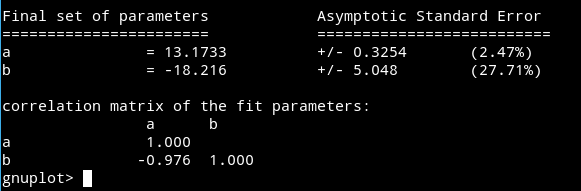
\includegraphics[scale=0.6]{ejercicio3/plot3-1.png}  
\caption{Cálculo de a y b} 
\label{fig:figura3-1}
\end{figure}

\begin{figure}[H] %con el [H] le obligamos a situar aquí la figura
\centering
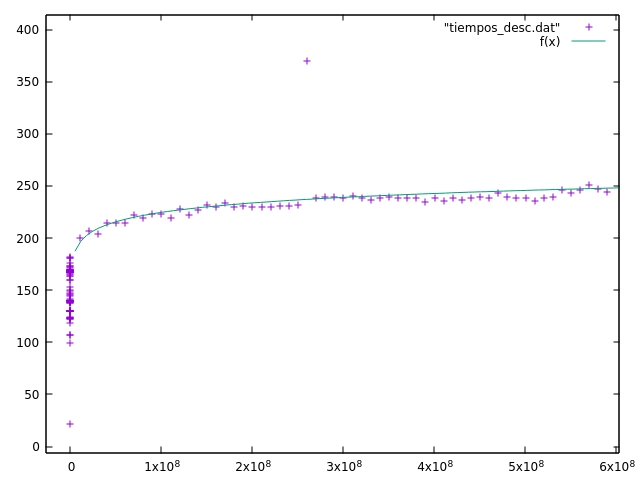
\includegraphics[scale=0.8]{ejercicio3/plot3-2.png}  
\caption{Regresión para ajustar la curva teórica a la empírica.} 
\label{fig:figura3-2}
\end{figure}

\end{enumerate}


\newpage
%------------------------------------------------

%----------------------------------------------------------------------------------------
%	Cuestión 4
%----------------------------------------------------------------------------------------
\section{Ejercicio 4: Mejor y peor caso}

Modificación del código para crear una situación de dos posibles casos.
\subsection{El mejor caso posible}
	
		Este caso es en el que el vector ya se encuentre ordenado. Para ello sólamente hay que modificar en el código la parte donde se rellena el vector después de su obligatoria reserva de espacio.
\begin {lstlisting}
// Generación del vector ORDENADO
int *v=new int[tam];       // Reserva de memoria
for (int i=0; i<tam; i++)  // Recorrer vector
	v[i] = i;    // Generar vector ya ordenado
	
\end{lstlisting}
	
\textbf{-- Eficiencia empírica}
\begin{figure}[H] %con el [H] le obligamos a situar aquí la figura
\centering
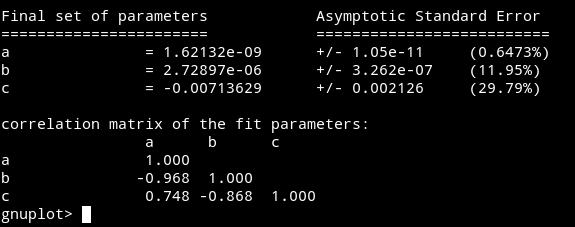
\includegraphics[scale=0.5]{ejercicio4/plotMejor.png}  
\caption{Cálculo de los parámetros.} 
\label{fig:figura4-1}
\end{figure}

\begin{figure}[H] %con el [H] le obligamos a situar aquí la figura
\centering
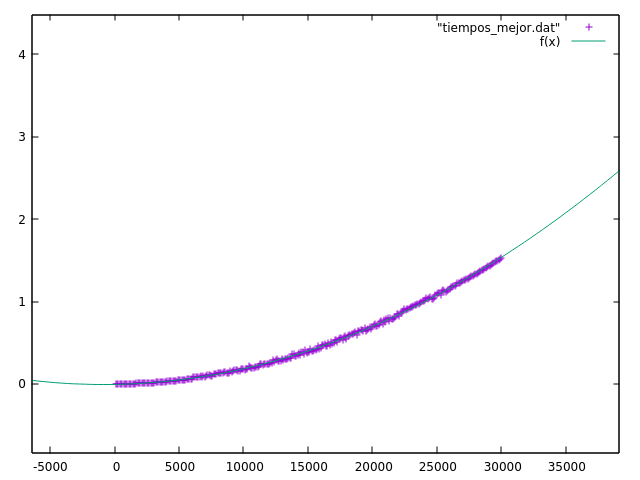
\includegraphics[scale=0.5]{ejercicio4/regresionMejor.png}  
\caption{Gráfica de la eficiencia empírica} 
\label{fig:figura4-2}
\end{figure}

\subsection{El peor caso posible}
	
		Este caso es en el que el vector ya se encuentre ordenado pero de manera inversa, es decir, el tamaño de los valores del vector irán de más a menos. Para ello sólamente hay que modificar en el código la parte donde se rellena el vector después de su obligatoria reserva de espacio.
\begin {lstlisting}
// Generación del vector ordenado del revés
int *v=new int[tam];       // Reserva de memoria
// Recorrer vector
for (int i=tam-1, j = 0 ; i >= 0 ; i--, j++)  
	v[i] = j;    // Generar vector ya ordenado
	
\end{lstlisting}

\textbf{-- Eficiencia empírica}
\begin{figure}[H] %con el [H] le obligamos a situar aquí la figura
\centering
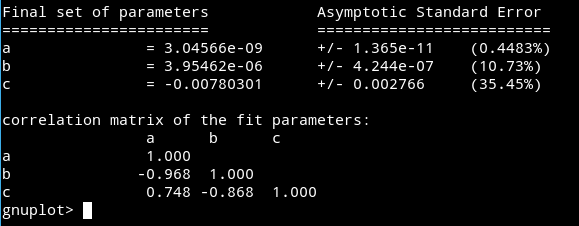
\includegraphics[scale=0.5]{ejercicio4/plotPeor.png}  
\caption{Cálculo de los parámetros.} 
\label{fig:figura4-3}
\end{figure}

\begin{figure}[H] %con el [H] le obligamos a situar aquí la figura
\centering
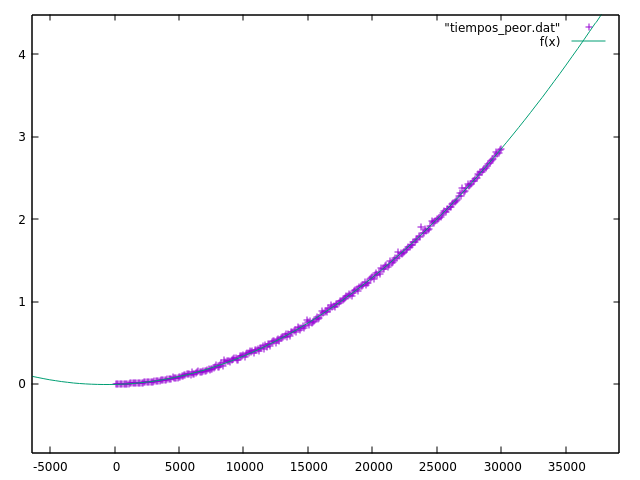
\includegraphics[scale=0.6]{ejercicio4/regresionPeor.png}  
\caption{Gráfica de la eficiencia empírica} 
\label{fig:figura4-4}
\end{figure}

\newpage
\subsection{Comparación de resultados}
Una vez obtenidos todos los resultados empíricos de la eficiencia se puede apreciar en la Figura~\ref{fig:figura4-5}, como era de esperar, que los tiempos con los resultados más eficientes son las del mejor caso y los menos, las del peor caso.
\begin{figure}[H] %con el [H] le obligamos a situar aquí la figura
\centering
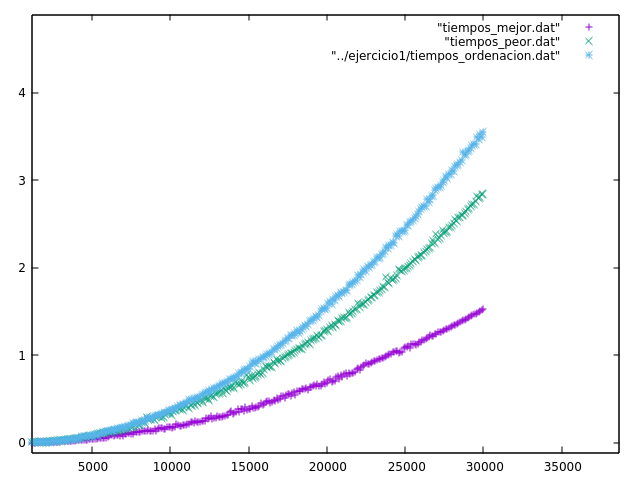
\includegraphics[scale=0.8]{ejercicio4/comparacionTodas.png}  
\caption{Comparación de resultados.} 
\label{fig:figura4-5}
\end{figure}

\newpage
%------------------------------------------------

%----------------------------------------------------------------------------------------
%	Cuestión 5
%----------------------------------------------------------------------------------------

\section{Ejercicio 5: Dependencia de la implementación}
\subsection{Cálculo de la eficiencia teórica del nuevo algoritmo de la burbuja}
\begin {lstlisting}
void ordenar(int *v, int n) {
    bool cambio=true;
    for (int i=0; i<n-1 && cambio; i++) {
        cambio=false;
        for (int j=0; j<n-i-1; j++)
            if (v[j]>v[j+1]) {
            /*Aquí nunca llegará con el bucle ordenado en el mejor caso*/
            }
    }
}
\end{lstlisting}

\begin{itemize}
	\item Linea 2: 1 OE (asignación)
	\item Linea 3: 4 OE (asignación, decremento, comparación, operación \&\&) + 1 OE	
	\item Linea 4: 1 OE (asignación)
	\item Linea 5: 4 OE (asignación, 2 decrementos, comparación) + 1 OE
	\item Linea 6: 4 OE (2 accesos al elemento v[j], incremento, comparación)
\end{itemize}
Al añadirse la variable booleana \textbf{cambio} se produce que, en el mejor de los casos, el orden de eficiencia teórico sea \textbf{O(n)}. Dicha variable sería siempre \textbf{false}, ya que la comparación que le precede también lo será por lo que el bucle externo se ejecuta una sola vez.

A continuación se realizará el estudio teórico del algoritmo.


\underline{Bucle de la j}
\begin{equation}
Tj(n)= \sum_{j=0}^{n-i-1}9 = 9n - 9i
\end{equation}

\begin{equation}
T(n)=1 + \sum_{i=0}^{1}(6 + 9n -9i) = 6 + \sum_{i=0}^{1}(9n) - \sum_{i=0}^{1}(9i) = 6+9n - 9 = 9n - 3
\end{equation}

Por lo que se puede confirmar que la eficiencia de la función es de \textbf{O(n)}

\newpage
\subsection{Cálculo de la eficiencia empírica del nuevo algoritmo de la burbuja}
\begin{figure}[H] %con el [H] le obligamos a situar aquí la figura
\centering
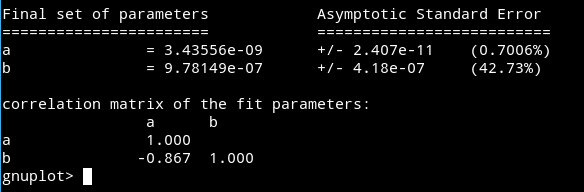
\includegraphics[scale=0.7]{ejercicio5/datosBurbuja.png}  
\caption{Cálculo de los parámetros.} 
\label{fig:figura5-1}
\end{figure}

\begin{figure}[H] %con el [H] le obligamos a situar aquí la figura
\centering
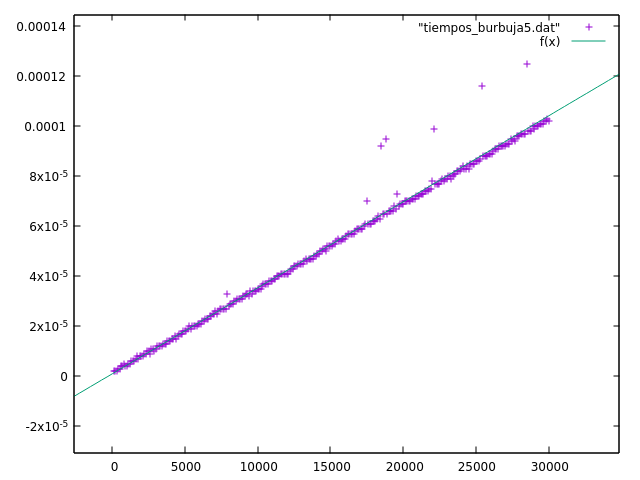
\includegraphics[scale=0.8]{ejercicio5/regresion.png}  
\caption{Gráfica de la eficiencia empírica.} 
\label{fig:figura5-2}
\end{figure}




\newpage
%------------------------------------------------

%----------------------------------------------------------------------------------------
%	Ejercicio 6
%----------------------------------------------------------------------------------------
\section{ADICIONAL - Ejercicio 6: Influencia del proceso de compilación}
\begin{figure}[H] %con el [H] le obligamos a situar aquí la figura
\centering
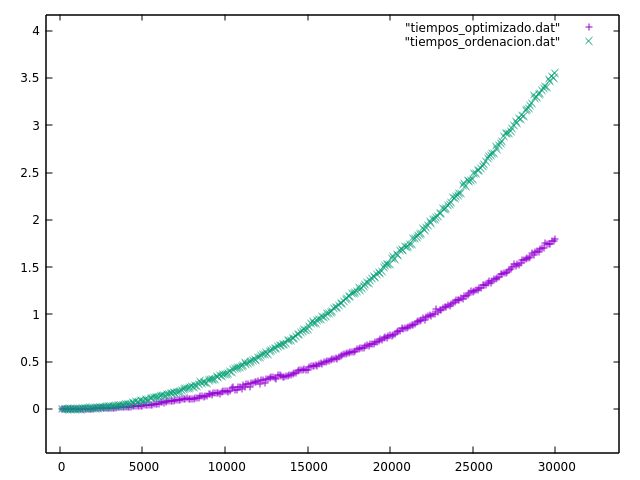
\includegraphics[scale=0.8]{ejercicio6/plot.png}  
\caption{Compilación normal VS optimizada.} 
\label{fig:figura6-1}
\end{figure}

\newpage
%------------------------------------------------

%----------------------------------------------------------------------------------------
%	Ejercicio 7
%----------------------------------------------------------------------------------------
\section{ADICIONAL - Ejercicio 7: Multiplicación matricial}
\lstinputlisting{ejercicio7/ejercicio7_matrices.cpp}
\subsection{Eficiencia teórica}
\begin {lstlisting}
for(int i = 0; i < tam; i++)
    for(int j = 0; j < tam; j++){
        R[i][j] = 0;
        for(int k =0 ; k < tam; k++)
            R[i][j]= R[i][j]+A[i][k]*B[k][j];
    }
\end{lstlisting}

\begin{itemize}
	\item Linea 1: 2 OE (asignación, comparación) + 1 OE
	\item Linea 2: 2 OE (asignación, comparación) + 1 OE	
	\item Linea 3: 2 OE (acceso al elemento R[i][j], asignación)
	\item Linea 4: 2 OE (asignación, comparación) + 1 OE
	\item Linea 5: 7 OE (4 accesos al elementos de las matrices, 2 operaciones, asignación)
\end{itemize}
Se tienen tres bucles anidados, haciendo cada uno \textbf{n iteraciones}. El resto de la función es de orden constante, por lo que puede identificarse cada una como \textbf{O(1)}. De esta forma, el tiempo de ejecución en función de n es:

\begin{equation}
T(n)=\sum_{i=0}^{n}\sum_{j=0}^{n}\sum_{k=0}^{n}1= \sum_{i=0}^{n}\sum_{j=0}^{n}n=n^3
\end{equation}
Por lo que se puede confirmar que la eficiencia de la función es de 
\begin{equation}
O(n^3)
\end{equation}


\newpage
\subsection{Eficiencia empírica}
\lstinputlisting{ejercicio7/ejecuciones_matrices.csh}
Al ser una función cúbica, como se descubrió anteriormente, se realiza la regresión a partir
de los parámetros obtenidos de la funcion 
\begin{equation}
f(x) = ax^3 + bx^2 + cx + d
\end{equation}

\begin{figure}[H] %con el [H] le obligamos a situar aquí la figura
\centering
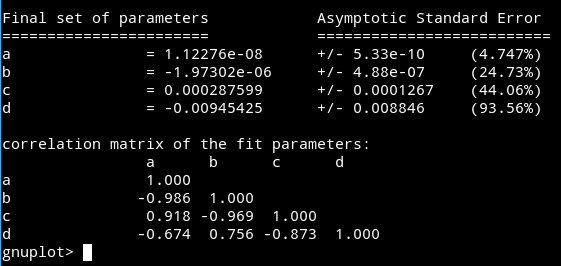
\includegraphics[scale=0.8]{ejercicio7/fit.png}  
\caption{Obtención de parámetros} 
\label{fig:figura7-1}
\end{figure}

\begin{figure}[H] %con el [H] le obligamos a situar aquí la figura
\centering
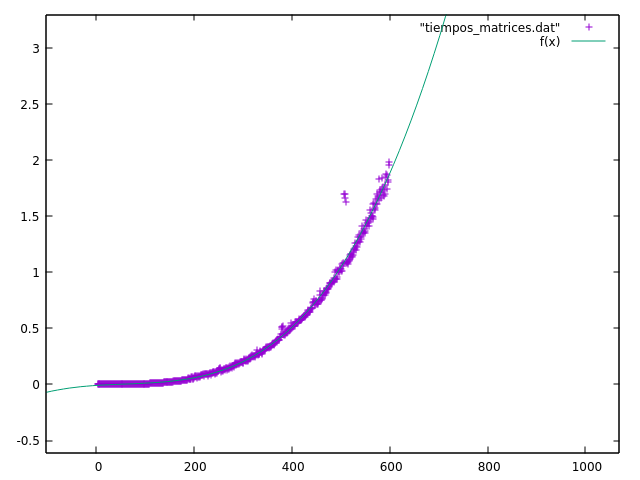
\includegraphics[scale=0.8]{ejercicio7/plot.png}  
\caption{Gráfico de la eficiencia empírica} 
\label{fig:figura7-1}
\end{figure}

\end{document}
